\chapter{Class Theory with Urelements}
This chapter studies class theory with urelements. In Section \ref{section:classwithurs}, I first introduce the axioms for class theory and show how urelement class theory can be interpreted in pure class theory. Then by generalizing the construction of class permutation models due to Felgner \cite{felgner1976choice}, I isolate a hierarchy of axioms in class theory with urelements. Section \ref{section:RP2withurelements} is concerned with the second-order reflection principle (RP$_2$) in Kelley-Morse class theory with urelements. I first show that when there are no more urelements than the ordinals, RP$_2$ with urelements is bi-interpretable with RP$_2$ in pure class theory. I then introduce a new form of accumulative hierarchy, $U_{\kappa, A}$, and prove a generalized version of Zermelo's Quasi-Categoricity Theorem with urelements. Assuming the consistency of a $\kappa^+$-supercompact cardinal, I construct a $U_{\kappa, A}$-model of RP$_2$ where the urelements are more numerous than the pure sets. At the end, I discuss how this result, together with my recent joint work with Hamkins \cite{HamkinsForthcoming-HAMRIS}, might challenge the doctrine of limitation of size.

\section{Class theory with urelements}\label{section:classwithurs}

\subsection{Axioms} \label{subsection:axiomsinclasstheory}
The language of \textit{ urelement class theory} is a two-sorted language extending the language of urelement set theory, with the first-order variables quantifying over sets and urelements, and the second-order variables quantifying over classes. Proper classes are classes that are not co-extensional with any set. A model for this language is of the form $\<M, \A^M, \in^M, \mathscr{M}>$, where the first-order part $\<M, \A^M, \in^M >$ is a model for the lanauge of urelement set theory and the second-order part $\mathscr{M} \subseteq P(M)$ serves as the domain for classes. In class theory, the axiom schemes in first-order set theory can be now written as single axioms.
\begin{itemize}
    \item [] (Separation) For every class $Y$ and set $x$, $Y \cap x$ is a set.
    \item [] (Replacement) If $F$ is a class function on a set $x$, $F[x]$ is a set.
    \item [] (Collection) If $R$ is a class relation on a set $w$ such that $\forall x \in w\ \exists y R(x, y)$, then there is a set $v$ such that for every $x \in w$ there is a $y \in v$ such that $R(x, y)$.
\end{itemize}
Similarly, for every $\kappa$, the DC$_\kappa$-scheme can be formulated as a single axiom, which I shall call ``$\kappa$-DC''.
\begin{itemize}
    \item [] ($\kappa$-DC) For every relation $R \subseteq U \times U$ that has no terminal nodes, there exists a function $f$ on $\kappa$ such that $R(f\restriction \alpha, f(\alpha))$ for all $\alpha < \kappa$.
 \end{itemize}
As in Proposition \ref{prop:DCkappaVariants}, $\kappa$-DC is equivalent to the assertion that for every class $X$, if every $s \in X^{<\kappa}$ has some $y \in X$ such that $R(s, y)$, then there is an $f \in X^\kappa$ such that $R(f\restriction \alpha, \alpha)$ for every $\alpha < \kappa$. $Ord$-DC is the statement that $\forall \kappa (\kappa$-DC). The same argument as in Lemma \ref{easyimplication} will show that $Ord$-DC holds when there is only a set of urelements over the theory $\GBUR$, which is defined below. The first-order reflection principle will now allow class parameters.
\begin{itemize}
    \item [] (RP) For every $X_1$, ..., $X_n$, there is a transitive set $t$ extending any given set such that for every $x_1, ..., x_m \in t$, $$\varphi(X_1, ..., X_n, x_1, ..., x_m) \leftrightarrow \varphi^t(X_1 \cap t, ..., X_n \cap t, x_1, ..., x_m),$$ where $\varphi$ contains only first-order quantifiers.
 \end{itemize}


Two standard theories of classes are G\"odel-Bernays class theory (GB) and Kelley-Morse class theory (KM). In addition to ZF for sets, GB adopts the following first-order comprehension axiom.
\begin{itemize}
\item [] (First-order Comprehension) For every formula $\varphi$ which contains only first-order quantifiers (but possibly with class parameters), $\{x : \varphi(x)\}$ is a class.
\end{itemize}
KM extends GB by adopting the full comprehension axiom.
\begin{itemize}
\item [] (Full Comprehension) For every formula $\varphi$, possibly with class parameters, $\{x : \varphi(x)\}$ is a class.
\end{itemize}
\noindent GB and KM  are often formulated with a second-order version of AC. However, in the presence of urelements different formulations of this principle can come apart. We shall discuss the following three versions.
\begin{itemize}
	\item[] (Limitation of Size) All proper classes are equinumerous.\footnote{It is immediate that Limitation of Size is equivalent to the following principle. \begin{itemize}
	    \item [] $X$ is a proper class if and only if it is equinumerous with the universe $U$.
	\end{itemize}
And this principle is precisely what the limitation-of-size conception of size (see \ref{subsection:philosophy}) is asserting, so the terminology here is justified.}
	\item[] (Global Well-Ordering) There is a well-ordering of the universe $U$.
	\item[](Global Choice) There is a class function $F$ such that for every non-empty set $x$, $F(x) \in x$.
\end{itemize}
Standard arguments show that over a suitable theory (such as the theory GBU$_\text{R}$ defined below), Limitation of Size $\rightarrow$ Global Well-Ordering $\rightarrow$ Global Choice. However, neither of the implications can be reversed, as proved in \cite{howard1978independence} (see also Theorem \ref{thm:KMURnvdashCollection} and Lemma \ref{UKA}). For this reason, it is useful to isolate urelement class theories that do not include any second-order choice principles.
\begin{definition}
\ \newline
GBU$_\text{R}$ $=$ ZU + Class Extensionality + Replacement + First-Order Comprehension.\\
KMU$_\text{R} =$ GBU$_\text{R}$ + Full Comprehension.\\
$\GBUR =$ GBU$_\text{R}$ + AC.\\
$\KMUR =$ KMU$_\text{R}$ + AC.\\
GBCU $=$ GBU$_\text{R}$ + Global Well-Ordering.\\
KMCU $=$ KMU$_\text{R}$ + Global Well-Ordering.\\
GBc $=$ $\GBUR + \forall x \neg \A (x) $\\
KMc $=$ $\KMUR + \forall x \neg \A (x)$\\
GBC $=$ GBCU  + $\forall x \neg \A (x) $.\\
KMC $=$ KMCU  + $\forall x \neg \A (x) $.
\end{definition}

Theories with a lowercase c do not include any second-order choice principle but only AC for sets. The subscript R indicates again that the theory is formulated with Replacement. As we will see in \ref{section:independenceinClassTheory}, neither $\omega$-DC nor Collection is provable from $\KMUR$, and Collection does not imply $\omega$-DC over $\KMUR$ (although Collection does imply the DC$_\omega$-scheme in $\ZFCUR$). Note that Limitation of Size was not included as an axiom for either KMCU or GBCU, and its philosophical status will be discussed in \ref{section:amodelofKMU+RP2+notLS}. Finally, Gitman and Hamkins \cite{GitmanHamkins:Kelley-MorseSetTheoryAndChoicePrinciplesForClasses} observed that a robust class theory should include the following principle of Class Choice. 
\begin{itemize}
    \item [] (CC) $\forall Z (\forall x \exists X \varphi(x, X, Z) \rightarrow \exists Y \subseteq U \times U \ \forall x \varphi(x ,Y_x, Z))$, where $Y_x = \{ y : \<x, y> \in Y \}$.
\end{itemize}
That is, if every $x$ has a class witness for some relation $\varphi$, there will be a two-dimensional class $Y$ whose $x$-slice is a class witness for $x$. For any cardinal $\kappa$, $\kappa$-CC is the following restricted version of CC.
\begin{itemize}
    \item [] ($\kappa$-CC) $\forall Z (\forall \alpha < \kappa\ \exists X \varphi(\alpha, X, Z) \rightarrow \exists Y \subseteq \kappa \times U \ \forall \alpha <\kappa\ \varphi(\alpha ,Y_\alpha, Z))$.
\end{itemize}
\noindent It is shown in \cite{GitmanHamkins:Kelley-MorseSetTheoryAndChoicePrinciplesForClasses} that even $\omega$-CC is not provable in KMC and that KMC and KMC + CC are mutually interpretable. 

I shall end this subsectoin with some useful facts, all of which should be well-known.
\begin{prop}\label{prop:GC<->GWO<->LS}
 Over GBU$_\text{R}$ + $\A$ is a set. The following are equivalent.
 \begin{enumerate}
     \item Limitation of Size.
     \item Global Well-Ordering.
     \item Global Choice.
 \end{enumerate}
\end{prop}
\begin{proof}
It is clear that over GBU$_\text{R}$, (1) $\rightarrow$ (2) $\rightarrow$ (3). To show (3) $\rightarrow$ (1), let $F$ be a global choice function. Define $G : Ord \rightarrow U$ as 
\begin{itemize}
    \item [] $G(0) = 0$;
    \item [] $G(\alpha) = F(V_\beta(\A) \setminus G[\alpha])$, where $\beta$ is the least ordinal such that $V_\beta(\A) \setminus G[\alpha]$ is non-empty.
\end{itemize}
It is not hard to verify that $G$ is a bijection and hence a global well-ordering. Now let $X$ be a proper class. As $\A$ is a set, the map from $X$ to $Ord$ that maps each $x \in X$ to its rank (i.e., the least $\beta$ such that $x \in V_\beta(\A)$) must be unbounded, which produces an onto map from $X$ to $Ord$. Since we can well-order $X$, there is an injective map from $Ord$ to X; and by a class version of the Cantor-Bernstein Theorem, it follows that $X$ and $Ord$ are equinumerous. Therefore, all proper classes are equinumerous. \end{proof}

\begin{prop}\label{prop:rp+gbur<->collection+dcs}
The following are equivalent over $\GBUR$.
\begin{enumerate}
    \item RP.
    \item Collection $\land \ \omega$-DC.
\end{enumerate}
\end{prop}
\begin{proof}
 To show (1) $\rightarrow$ (2), assume RP. Suppose that $\forall x \in w\ \exists y\  R(x, y)$ for some class relation $R$ and set $w$. We can then reflect it down to a transitive set extending $w$, which will give us a collection set. And suppose that $R$ is a class relation without terminal nodes; we can then reflect this fact down to some transitive set $t$. The existence of a desired $\omega$-sequence then follows from AC. (2) $\rightarrow$ (1) is proved in the same way as in Theorem \ref{collection+dc->rp} since the class parameters do not raise any difficulties.
\end{proof}

\begin{prop}\label{prop:OrdDC->RP}
  GBU$_\text{R} + Ord$-DC $\vdash$ RP.
\end{prop}
\begin{proof}
Assume $Ord$-DC. By a standard argument as in \cite[Theorem 8.1]{jech2008axiom}, $Ord$-DC implies AC. Also, by Proposition \ref{prop:rp+gbur<->collection+dcs}, it suffices to show that Collection holds. Let $w$ be an infinite set and $R$ be a class relation such that $\forall x \in w\ \exists y\  R(x, y)$. We may enumerate $w$ with $\{x_\alpha : \alpha < \kappa\}$ by some infinite cardinal $\kappa$. Define $X = \{ \<x_\alpha, y> : \alpha < \kappa \land R(x_\alpha, y) \}$. For every $s$ and $z$, define
\begin{itemize}
    \item []  $R^*(s, z)$ if and only if, whenever $s$ is function on $\alpha$ for some $\alpha < \kappa$, $z = \<x_\alpha, y>$ and $z \in X$.
\end{itemize}
 By $Ord$-DC, there is an $f \in X^\kappa$ such that $R^*(f\restriction \alpha, f(\alpha))$ for every $\alpha < \kappa$. Then the transitive closure of $f$ will be a desired collection set.  
\end{proof}

\begin{prop}\label{prop:GBU->RPandDCord}
GBCU $\vdash$ $Ord$-DC $\land$ RP.
\end{prop}
\begin{proof}
Given a class relation without terminal nodes, for every $\kappa$ we can use the global well-ordering to construct a desired $\kappa$-sequence. Then RP holds by Proposition \ref{prop:OrdDC->RP}.
\end{proof}
To conclude, the following diagram holds in $\GBUR$, whose completeness will be discussed in \ref{section:independenceinClassTheory}.
\begin{figure}[hbt!]
\begin{center}
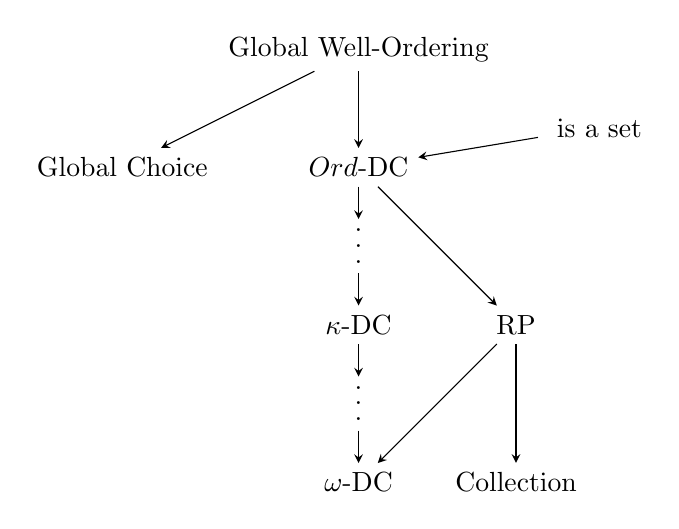
\begin{tikzpicture}
\begin{scope}[every node/.style={}]
    \node (A) at (8, -2.5) {Collection};
    \node (B) at (9, 2){$\A$ is a set};
    \node (C) at (3, 1.5){Global Choice};
    \node (D) at (6,1.5) {$Ord$-DC };
    \node (E) at (6, -0.5) {$\kappa$-DC};
    \node (I) at (8, -0.5) {RP};


    \node (L) at (6, 0.7) {.};
    \node (M) at (6, 0.5) {.};
    \node (N) at (6, 0.3) {.};
    \node (P) at (6, -1.7) {.};
    \node (Q) at (6, -1.5) {.};
    \node (R) at (6, -1.3) {.};
    \node (S) at (6, -2.5) {$\omega$-DC};
    \node (T) at (6, 3) {Global Well-Ordering};
    
\end{scope}

\begin{scope}[>={stealth},
              every node/.style={fill=white,circle},
              every edge/.style={draw=black}]

    \path [->] (T) edge (D);
\path [->] (T) edge (C);
     \path [->] (B) edge (D);
     


    \path [->] (I) edge (A);
      \path [->] (I) edge (S);
    \path [->] (D) edge (I);
    \path [->] (D) edge (L);
    \path [->] (N) edge (E);
    \path [->] (E) edge (R);
     \path [->] (P) edge (S);
       
\end{scope}
\end{tikzpicture}
 \caption{Implication diagram in $\GBUR$}
 \label{GBUdiagram}
\end{center}
\end{figure}
\FloatBarrier
\subsection{Interpreting $\mathcal{U}$ in $\mathcal{V}$}\label{section:interpretingUrelementsinClassTheory}
The construction of $V\llbracket X \rrbracket$ introduced in Section \ref{section:interpretingUinV} can be easily generalized to interpreting urelement class theory in pure class theory.
\begin{definition}\label{barwiseinterpretation2}
Let $\<V, \in , \mathscr{V}>$ be a model of GBc and $X \in \mathscr{V}$. $\<V \llbracket X \rrbracket, \bar{A}, \bar{\in}>$ is then defined as in Definition \ref{barwiseinterpretation1}. Let $\mathscr{V}\llbracket X \rrbracket = \{Y \in \mathscr{V} : Y \subseteq  V \llbracket X \rrbracket\}$. $\mathscr{V}\llbracket X \rrbracket$ denotes the model $\< V \llbracket X \rrbracket, \bar{A}, \bar{\in}, \mathscr{V}\llbracket X \rrbracket>$.\footnote{Note that when $Y \in \mathscr{V}\llbracket X \rrbracket$, $\mathscr{V}\llbracket X \rrbracket \models x \in Y$ if and only if $\mathscr{V} \models x \in Y$.}
\end{definition}

\begin{theorem}\label{Con(KM)->Con(KMU)}
Suppose $\mathscr{V} \models $ GBc and $X$ is a class in $\mathscr{V}$. Then
\begin{enumerate}
    \item $\mathscr{V}\llbracket X \rrbracket \models $ $\GBUR$ + Collection;
    \item $\mathscr{V}\llbracket X \rrbracket \models $ $\KMUR$ + Collection if $\mathcal{V} \models$ KMc;
    \item $\mathscr{V}\llbracket X \rrbracket \models $ CC if $\mathscr{V} \models$ CC;
    \item $\mathscr{V}\llbracket X \rrbracket \models $ Limitation of Size (and hence GBCU) if $\mathcal{V} \models$ GBC.
\end{enumerate}
\end{theorem}

\begin{proof}


For (1) and (2), $\mathscr{V}\llbracket X \rrbracket \models$ ZU by Theorem \ref{thm:V[X]modelsZFU}, so it remains to show that $\mathscr{V}\llbracket X \rrbracket$ satisfies Collection, Class Extensionality, and First-Order Comprehension (or Full Comprehension), all of which follow easily from the fact that $\mathscr{V} \models$ GBc (or KMc). For example, to show $\mathscr{V}\llbracket X \rrbracket \models$ Collection, suppose that in $\mathscr{V}\llbracket X \rrbracket$ for every $x \in \barw$ there is some $y$ such that $x \bar{R} y$ for some $\barw, \bar{R} \in \mathscr{V}\llbracket X \rrbracket$, where $\barw = \<1, w>$. Then in $V$ there is some $v \subseteq V \llbracket X \rrbracket$ such that for every $\barx \in w$, there is some $\bary \in v$ such that $\mathscr{V}\llbracket X \rrbracket \models \<\barx, \bary> \in \bar{R}$. Then $\bar{v} = \<1, v>$ is a desired collection set in $\mathscr{V}\llbracket X \rrbracket$.

(3) Suppose that $\mathscr{V} \models$ CC AND for every $\barx \in V\llbracket X \rrbracket$, there is some class $\bar{X} \in \mathscr{V}\llbracket X \rrbracket$ with $\varphi(\barx, \bar{X}, \bar{Z})^{ \mathscr{V}\llbracket X \rrbracket}$. By CC in $\mathscr{V}$, there is a class $Y \subseteq V\llbracket X \rrbracket \times U$ such that for every $\barx \in V\llbracket X \rrbracket$, $\varphi(\barx, Y_{\barx}, \bar{Z})^{ \mathscr{V}\llbracket X \rrbracket}$ and $Y_{\barx} $ is a class of $\mathscr{V}\llbracket X \rrbracket$. Define $\overline{Y} = \{\overline{\<\barx, \bary>} : \bary \in Y_{\barx} \land \barx \in \mathscr{V}\llbracket X \rrbracket \}$ (where $\overline{\<\barx, \bary>}$ codes the ordered-pair as in Theorem \ref{thm:ACholdsViffACholdsinV[X]}), which is a class of $\mathscr{V}\llbracket X \rrbracket$. Since for every $\barx \in \mathscr{V}\llbracket X \rrbracket$, $\mathscr{V}\llbracket X \rrbracket \models Y_{\barx} = \overline{Y}_{\barx}$, it follows that CC holds in $\mathscr{V}\llbracket X \rrbracket$.

(4) Suppose that $\mathscr{V}$ Global Well-Ordering. Note that if $\bar{Y}$ and $\bar{Z}$ are two proper classes in $\mathscr{V}\llbracket X \rrbracket$ , they must be equinumerous proper classes in $\mathscr{V}$ by Propostion \ref{prop:GC<->GWO<->LS}. So in $\mathscr{V}$ there must be a bijection $F$ between $\bar{Y}$ and $\bar{Z}$. Then $\bar{F} = \{ \overline{\<\bary, \barz>} : F(\bary) = \barz \}$ will be a bijection between $\bar{Y}$ and $\bar{Z}$ in $\mathscr{V}\llbracket X \rrbracket$.\end{proof}


\begin{theorem}\label{KMU+LSbiintepsKM+LS}
The following pairs of theories are bi-interpretable with parameters.
\begin{enumerate}
    \item GBC and GBCU + $\A \sim \omega$;
    \item KMC and KMCU + $\A \sim \omega$;
    \item GBC and GBCU + Limitation of Size;
    \item KMC and KMCU + Limitation of Size;
    \item GBC and GBCU + Limitation of Size + Plenitude;
    \item KMC and KMCU + Limitation of Size + Plenitude.
\end{enumerate}
\end{theorem}
\begin{proof}
Working in GBC (KMC), we can form either $\mathscr{V}\llbracket \omega \rrbracket$ (or $V\llbracket Ord\rrbracket$), and the map $y \mapsto \hat{y}$ and $Y \mapsto \hat{Y} = \{\hat{y} : y \in Y\}$ will be a definable isomorphism between $\mathcal{V}$ and $V^{\mathcal{V}\llbracket \omega \rrbracket}$ (or $V^{\mathcal{V}\llbracket Ord \rrbracket}$). In KMCU + Limitation of Size, there will be an injective map $F$ from $\A$ to $V$. For every urelement $a$, let $\tilde{a} = \<0, F(a)>$; and for every set $x$, we let $\tilde{x} = \<1, \{\tilde{y} : y \in x\}>$. It follows by an easy induction that the map $x \mapsto \tilde{x}$ and $X \mapsto \tilde{X} = \{\tilde{x} : x \in X\}$ is an isomorphism between $U$ and $V\llbracket F[\A] \rrbracket$.
\end{proof}

\begin{corollary}\label{corollary:LS<->AlessthanV}
Over KMCU, the following are equivalent.
\begin{enumerate}
    \item Limitation of Size.
    \item There is an injective map from $\A$ to $V$.
\end{enumerate}
\end{corollary}
\begin{proof}
(1) $\rightarrow$ (2) is clear. For (2) $\rightarrow$ (1), first observe that over KMCU, Limitation of Size holds for the pure classes $\mathcal{V}$. For, given a global choice function, its restriction to $V$ is a pure class so $\mathcal{V} \models $ Global Choice, which means $\mathcal{V} \models $ Limitation of Size by Proposition \ref{prop:GC<->GWO<->LS}. Now suppose that $F$ is an injective map from $\A$ to $V$. Since $U$ and $V\llbracket F[\A] \rrbracket$ are equinumerous, every proper class is equinumerous with a pure proper class. Therefore, all proper classes are equinumerous.
\end{proof}

\subsection{Independence results}\label{section:independenceinClassTheory}
In this subsection, I discuss several independence results concerning the completeness of Diagram \ref{GBUdiagram} over $\KMUR$. To begin with, arguments in \ref{subsection:implicationdiagram} which appeal to homogeneity can no longer go through in the context of class theory. For example, one might attempt to show that $\KMUR$ + Plenitude implies $\omega$-DC by the same argument as in Theorem \ref{Plenitude->DCS}. But the problem is that the ``kernel'' of a class relation $R$ might be a proper class, in which case we cannot find some a set of urelements that is big enough to ``fix'' $R$. In fact, we will see that over $\KMUR$,
\begin{enumerate}
    \item $\kappa$-DC $\nrightarrow$ Collection;
    \item Global Choice  $\nrightarrow$ ($\omega$-DC $\lor$ Collection);
    \item Collection $\nrightarrow$ $\omega$-DC;
    \item RP $\nrightarrow$ $\omega_1$-DC.
\end{enumerate}
Since it is well-known that KMc cannot prove Global Well-Ordering, it follows that Diagram \ref{GBUdiagram} is indeed complete over $\KMUR$.

Let me first discuss a general method of constructing \textit{class permutation models} of $\KMUR$ used in \cite{felgner1976choice}. Given a model $\<U, \A, \in, \U>$ of KMCU, we might fix an $\A$-ideal $\I$ as in Definition \ref{normalideal} and consider $U^\I$, the class of all first-order objects whose kernel is small in the sense of $\I$. This will give us a model of $\ZFCUR$ as before. To have a model of $\KMUR$, however, we cannot take all subclasses of $U^I$ as the second-order part of $U^\I$. To see this, suppose that $\A$ is an infinite set and $\I$ is its ideal of finite subsets; then an injection $F$ from $\omega$ to $\A$ will be a subclass of $U^\I$, which means having $F$ as a class of the model we intend to build would violate Replacement. In other words, we need to throw out some subclasses of $U^\I$. This is done by finding some suitable group $\G$ of permutations on $\A$ and only keep those subclasses of $U^\I$ that are \textit{symmetric} with respect to $\I$ and $\G$.

\begin{definition}[KMCU]
Let $\G$ be a group of permutations of $\A$.\footnote{It is understood that every $\pi \in \G$ is a permutation of a \textit{set} of urelements. Whenever $\pi, \sigma \in \G$, $\pi \circ \sigma$ is taken as the composition of their canonical extensions, which point-wise fix the urelements not in their original domains.} For any $x \in U$, $sym(x)$ and $fix(x)$ are defined as in Definition \ref{permutationmodeldef}. Let $\I\in \U$ be an $\A$-ideal as in Definition \ref{normalideal}. $\I$ is said to be $\G$-\textit{flexible} if 
\begin{enumerate}
    \item for every $\pi \in \G$ and $A \in \I$, $\pi A \in \I$;
    \item $\I$ has a \textit{basis} such that for every $B$ in the basis and $ A \in \I$ disjoint from $B$, there is some $\pi \in fix(B)$ such that $\pi A \neq A$.
\end{enumerate}
A class $X$ is \textit{symmetric} (w.r.t. $\G$ and $\I$) if there is some $A \in \I$, called a \textit{support} of $X$, such that $fix(A) \subseteq sym(X)$, where $sym(X) = \{\pi \in \G : \pi X = X\}$.  $U^\I =\{ x\in U : ker(x) \in \I\}$. $\W = \{ X \subseteq U^\I : X \text{ is symmetric}\}$. The model $\<U^\I, \in, \A, \W>$ is also denoted by $\W$.
\end{definition}
\noindent As we shall see later, $\G$-flexibility ensures that enough classes are thrown out so that Replacement can hold in $\W$. It is easy to check that every $\pi \in \G$ is an automorphism of $\W$ because $\I$ is $\G$-flexible.

\begin{theorem}[KMCU]\label{classpermutationmodel}
Let $\G$ be a group of permutations on $\A$ and $\I$ be an $\A$-ideal that is $\G$-flexible. Then $\W \models \KMUR$. 
\end{theorem}
\begin{proof}
$\W$ is a transitive class containing all the urelements and pure sets. And by the same argument as in Theorem \ref{smallkernelmodel}, it follows that $\W \models $ ZU + AC + Separation + Class Extensionality.  


To show $\W \models$ Replacement, suppose that $x \in \W$ be a set and $F \in \W$ be a class function on $x$ with a support $A \in \I$. Let $\mathcal{J}$ be a basis of $\I$ which witnesses its flexibility and $B$ be a set of urelements in $\J$ with $ker(x) \cup A \subseteq B$. It suffices to show that $ker(F[x]) \subseteq B$. If not, then there is some $y \in F[x]$ such that $ker(y) \setminus B$ is not empty. Since $ker(y) \setminus B \in \I$, it follows that there is some $\pi \in fix(B)$ such that $\pi (ker(y) \setminus B) \neq ker(y) \setminus B$, and as a result, $\pi y \neq y$. But $F(z) = y$ for some $z \in x$ so $F(z) = \pi y$, which is a contradiction.


To show that Full Comprehension holds in $\W$, fix a formula $\varphi$ in the language of urelement class theory and classes $X_0, .., X_n \in \W$, in $\U$ let $X = \{ x \in  \W: \W \models \varphi (x, X_0, ... ,X_n \}$. It suffices to show that $sym(X_0) \cap ... \cap sym(X_n) \subseteq Sym(X)$. Fix a $\pi \in sym(X_0) \cap ... \cap sym(X_n)$. For every $x \in X$, since $\pi$ is an automorphism of $\W$, it follows that $\W \models \varphi (\pi x, X_0, ..., X_n)$ and hence $\pi x \in X$. Therefore, $\pi X = X$.
\end{proof}
\begin{theorem}\label{thm:KMUR+kDCvdashCollection}
Assume the consistency of KM. Let $\kappa$ be any infinite cardinal. There is a model of $\KMUR$ in which
\begin{enumerate}
    \item $\kappa$-DC holds;
    \item Collection fails.
\end{enumerate}
\end{theorem}
\begin{proof}
Let $\U$ be a model of KMCU + $\A \sim \aleph_{\kappa^+}$. Let $\I$ be the ideal of all sets of urelements of size less than $\aleph_{\kappa^+}$ and $\G$ be the group of all permutations of $\A$. It is clear that $\I$ is $\G$-flexible, so the resultant model $\W$ satisfies $\KMUR$. Collection fails in $\W$ because every cardinal below $\aleph_{\kappa^+}$ is realized while $\aleph_{\kappa^+}$ is not. To show $\kappa$-DC holds in $\W$, suppose that $R$ is a class relation in $\W$ without terminal nodes. Since the first-order domain of $\W$, $U^\I$, is closed under $\kappa$-sequences, $\U$ thinks that $\forall s \in (U^\I)^{<\kappa} \exists y \in U^\I R(x, y)$; by $Ord$-DC in $\U$, it follows that there is an $f \in (U^\I)^{\kappa}$ such that $R(f\restriction \alpha, f(\alpha))$ for every $\alpha < \kappa$. $f$ lives in $U^\I$, so $\kappa$-DC holds in $\W$.
\end{proof}


\begin{theorem}[Felgner \cite{felgner1976choice}]\label{thm:KMURnvdashCollection}
Assume the consistency of KM. There is a model of $\KMUR$ in which
\begin{enumerate}
    \item Global Choice holds;
    \item $\omega$-DC fails;
    \item Collection fails.
\end{enumerate}
\end{theorem}
\begin{proof}
Let $\U$ be a model of KMCU + $\A \sim \omega$, in which we identify $\A$ with the rationals $\<\Q, <_\Q>$. Let $\G$ be the group of permutations of $\A$ that preserves $<_\Q$ and $\I$ be the ideal of finite subsets of $\A$. $\I$ is $\G$-flexible: if $A, B \in \I$ are disjoint, for any $b \in B \setminus A$, there is an open interval containing $b$ that is disjoint from $A \cup B \setminus \{b\}$; so we can permute this interval in an order-preserving way and leave $A$ point-wise fixed. By Theorem \ref{classpermutationmodel}, it follows that the resultant class permutation model $\W$ satisfies $\KMUR$. Moreover, both Collection and $\omega$-DC fail in $\W$ since there is a proper class of urelements but every set of them is only finite. For a proof of $\W \models$ Global Choice, see \cite[pp. 249-250]{felgner1976choice} or \cite[Lemma 2.3]{yao2022reflection}. \end{proof}

\begin{theorem}\label{kmudoesnotproveDC}
Assume the consistency of KM. There is a model of $\KMUR$ in which 
\begin{enumerate}
    \item Collection holds;
    \item Plenitude holds;
    \item $\omega$-DC fails.
\end{enumerate}
\end{theorem}

\begin{proof}
The model used here is also due to Felgner\cite{felgner1976choice}. The point here is that the model also satisfies Collection, which is not discussed in Felgner's paper. Let $\U$ be a model of KMCU with an enumeration of $\A$ with the tree $Ord^{<\omega}\setminus \{\emptyset\}$ consisting of all non-empty finite sequences of ordinals. Each urelement is identified with a node on the tree and define $a \lhd b$ as $a \subsetneq b$. $b$ is said to be an \textit{immediate descendant} of $a$ if $b$ extends $a$ by one digit. $b$ and $b'$ are \textit{siblings} if either they are both top nodes, or they are an immediate descendant of the same node. A set $t \subseteq \A$ is a \textit{tree} if it is closed under initial segment (i.e, if $b \in t$ and $a \lhd b$, then $a \in t$). A \textit{path} of a tree $t$ with length $\alpha$ is a function $f: \alpha \rightarrow Ord$ such that $f\restriction \beta \in t$ for all $\beta < \alpha$. A \textit{branch} is a maximal path, i.e., it is not properly extended by any path of the tree. A tree $t$ is \textit{small} if it has no infinite branch. Let $\T$ be the class of all small trees, which forms a basis for an ideal $\I$. Let $\G$ be the group of  permutations of $\A$ that preserves $\lhd$.
\begin{lemma}\label{treeflexible}
$\I$ is $\G$-flexible with respect to the basis $\T$.
\end{lemma}
\begin{proof}
If $a$ and $b$ are siblings with domain $n + 1$, then there is a natural permutation $\pi^a_b \in \G$ such that for every node $c$ with $dom(c) = j +1$ and $i < j+1$,
\begin{equation*}
   \pi^a_b c (i)  =
    \begin{cases*}
      b(n) & if $i = n$, $c(n) = a(n)$ and $c \restriction n = a \restriction n$  \\
      a(n) & if $i = n$, $c(n) = b(n)$ and $c \restriction n = a \restriction n$  \\
      c(i) & otherwise
    \end{cases*}
 \end{equation*}
 $\pi^a_b$ thus swaps only $a$ and $b$ and their descendants. Given a small tree $t$ and some $A \in \I$ disjoint from $t$, since every node has  $Ord$-many siblings we can find a node $a$ in $A$ and a sibling $b$ of $a$ such that $b \notin t \cup A$. $\pi^a_b$ will then leave $t$ point-wise fixed because $t$ is a tree.
\end{proof}
\noindent Therefore, the class permutation model $\W$ given by $\G$ and $\I$ satisfies $\KMUR$. $\W$ clearly satisfies Plenitude because for every $\kappa$, there are $\kappa$-many top nodes on the tree $Ord^{<\omega}\setminus \{\emptyset\}$. Suppose \textit{for reductio} that $\omega$-DC holds in $\W$. Since in $\W$ every $a \in \A $ has some $b \in A$ such that $a \lhd b$, then in $\W$ there is an infinite branch $s = \<a_n : n < \omega>$ such that $a_n \lhd a_{n+1}$ for every $n$. Let $t$ be a small tree such that $fix(t) \subseteq sym(s)$. Fix some $a_n$ not in $t$ and some sibling $b$ of $a_n$ such that $b \notin t$. Then $\pi_{a_n, b} \in fix(t)$ but $\pi_{a_n, b} (s) \neq s$, which is a contradiction.

It remains to show that $\W \models$ Collection. For any two small tress $t$ and $t'$, we say that $t$ \textit{mildly extend} $t'$ if $t' \subseteq t$ and no branch of $t$ properly extends a branch of $t'$.


\begin{lemma}\label{treelemma}
Let $t_0, t_1 \in \T$ be such that $t_0 \subseteq t_1$ and every terminal node in $t_0$ has a descendent in $t_1$. Then for every $t \in \T$, there is a $\pi \in fix(t_0)$ such that $ t_1 \cup \pi t $ mildly extends $t_1$.  
\end{lemma}
\begin{proof}
Define $M = \{ a \in t_1 \setminus t_0 : a \text{ is an initial node in } t_1 \setminus t_0 \text{ and } a \text{ has a descendant in } t\}$, where ``$a$ initial in $t_1 \setminus t_0$'' means there is no node $b \in t_1 \setminus t_0$ such that $b \lhd a$. Since every node has $Ord$-many siblings and Global Well-Ordering holds in $\U$, for every $a \in M$ we can pick a sibling $a'$ of $a$ such that $a' \notin t_1 \cup t$, and we can ensure that $a_1' \neq a_2'$ for any distinct  $a_1, a_2 \in M$. Let $\pi = \bigcup_{a \in M}\pi^a_{a'}$, which is in $\G$. $\pi \in fix(t_0)$, because no node in $t_0$ is a descendant of any node in $M$ and $\pi$ only moves nodes in $M$ and their descendants.

To show that $t_1 \cup \pi t $ mildly extends $t_1$, consider any branch $f$ of $t_1$. Suppose \textit{for reductio} that $f$ is properly extended by a branch $g$ of $\pi t$. Note that $f$ must contain a node not in $t_0$ since otherwise $f$ would be a branch of $t_0$, which is impossible because every branch of $t_0$ is properly extended by a branch of $t_1$. So let $a$ be the least such node. There is a node $b$ on $g$ such that $a \lhd b$, where $b =\pi c$ for some $c \in t$. It follows that $a$ must be in $M$. If not, then $\pi a = a$ so $a \lhd c$ and hence $a$ is in $M$ after all. Thus, $\pi a = a'$ for some $a' \notin t$, but then $a' \lhd c$ so $a' \in t$---contradiction.
\end{proof}

\begin{lemma}
For any infinite cardinal $\kappa$, if $\<t_\alpha : \alpha < \kappa>$ is a sequence of small trees such that $t_\alpha$ mildly extends $\bigcup_{\beta < \alpha} t_\beta$ for every $\alpha < \kappa$, then $\bigcup_{\alpha < \kappa} t_\alpha$ is a small tree.
\end{lemma}
\begin{proof}
Let $t= \bigcup_{\alpha < \kappa} t_\alpha$. Suppose \textit{for reductio} that $f$ is an infinite branch of $t$. There will be some $t_\alpha$ with some $0 < m < \omega$ such that $f\restriction m$ is a branch of $t_\alpha$. Then for some $\beta > \alpha$, $t_\beta$ contains a branch that extends $f \restriction m$, which contradicts the assumption.
\end{proof}

Now suppose that $\W \models \forall x \in w \exists y \<x, y> \in R$ for some $w, R \in \W$. Let $t_0$ be a small tree that includes $ker(w)$ and some support of $R$, and enumerate $w$ by $\{x_\alpha : \alpha <\kappa\}$ for some $\kappa$. In $U$, we define a $\kappa$-sequence of small tress $\<t_\alpha : \alpha < \kappa>$ such that 
\begin{itemize}
    \item [] (i) $t_\alpha$ mildly extends $\bigcup_{\beta < \alpha} t_\beta$ for every $\alpha < \kappa$;
    \item [] (ii) for each $x_\alpha$, there is some $y \in \W$ such that $\<x_\alpha, y> \in R$ and $ker(y) \subseteq  t_\alpha$.
\end{itemize}
This is possible, because for every $x_\alpha$, fix some $y'$ with $\<x, y'> \in R$. Since $ker(y')$ is a subset of some small tree $t$, by Lemma \ref{treelemma}, there is a $\pi \in fix (t_0)$ such that $\bigcup_{\beta < \alpha} t_\beta \cup \pi t$ mildly extends $\bigcup_{\beta < \alpha} t_\beta$. Thus $\<x_\alpha, \pi y'> \in R$ and $ker(\pi y') \subseteq \pi t$. Let $t_\kappa = \bigcup_{\alpha < \kappa} t_\alpha$, which is a small tree. It follows that $\forall x \in w \exists y \in V(t_\kappa) \ (\<x, y> \in R)$, which suffices for Collection in $\W$.
\end{proof}
\noindent By using the same argument at the previous theorem, it is not hard to show that $\W \models \kappa$-CC for every infinite cardinal $\kappa$. However, it is unclear if the model $\W$ in Theorem \ref{kmudoesnotproveDC} satisfies CC if we assume $\U \models$ CC. 


\begin{theorem}\label{thm:RPnvdashOmega1Dc}
Assume the consistency of KM. There is a model of $\KMUR$ in which 
\begin{enumerate}
    \item RP holds;
    \item Plenitude holds;
    \item $\omega_1$-DC fails.
\end{enumerate}
\end{theorem}
\begin{proof}
Let $\U$ be a model of KMCU with an enumeration of $\A$ with the tree $Ord^{<{\omega_1}}\setminus \{\emptyset\}$ consisting of all non-empty \textit{countable} sequences of ordinals. A set $t$ of urelements is an $\omega_1$-small tree if it is a tree without any $\omega_1$-branch. Let $\I$ be the ideal generated by all the $\omega_1$-small trees and $\G$ be the group of permutations of $\A$ that preserve the tree structure as in the proof of Theorem \ref{kmudoesnotproveDC}. Since the same arguments in Lemma \ref{treeflexible} and \ref{treelemma} still go through, it follows that $\I$ is $\G$-flexible and that Collection holds in the resultant model $\W$.
\begin{claim}
$\W \models $ RP. 
\end{claim}
\begin{claimproof}
By Proposition \ref{prop:rp+gbur<->collection+dcs}, it is enough to show that $\omega$-DC holds in $\W$. So it suffices to show that the ideal $\I$ is countably closed. This is simply because the union countably many $\omega_1$-small trees, $\{t_n : n< \omega \}$, is an $\omega_1$-small tree. 
\end{claimproof}
\begin{claim}
$\W \models $ $\neg$($\omega_1$-DC).
\end{claim}
\begin{claimproof}
Suppose \textit{for reductio} that $\omega_1$-DC holds in $\W$. Say that a sequence $s \in \A^\alpha$ is a \textit{chain} if $s(\beta) \lhd s(\beta')$ for every $\beta < \beta' < \alpha$; and $s$ is said to be \textit{bound} by $a$ if $s(\beta) \lhd a$ for every $\beta < a$. In $\W$, every chain $s\in \A^{<\omega_1}$ has a bound $a \in \A$. By  $\omega_1$-DC, in $\W$ there is an $f \in \A^{\omega_1}$ that is a chain of length $\omega_1$. Then $ker(f)$ must be contained in some $\omega_1$-small tree, which is impossible.
\end{claimproof}

\end{proof}

\subsection{Open questions}
It is a classic result that GBC is a conservative extension of ZFC (e.g., see \cite{felgner1976choice}). But we know that GBCU is \textit{not} a conservative extension of ZFCU: GBCU proves that either $\A$ is a set, or Plenititude holds, which is not provable in ZFCU.
\begin{question}
\
\begin{enumerate}
    \item Is $\GBUR$ + Global Choice conservative over $\ZFCUR$?
    \item Is $\GBUR$ + Collection + Global Choice conservative over ZFCU?
\end{enumerate}
\end{question} 
\noindent Given Theorem \ref{kmudoesnotproveDC} and the fact that CC is a stronger version of Collection, it is natural to ask the following.
\begin{question}
Does $\KMUR$ prove any of the following?
\begin{enumerate}
    \item Collection $\land$ Global Choice $\rightarrow$ $\omega$-DC.
    \item CC $\rightarrow$ $\omega$-DC.
    \item CC $\land$ Global Choice $\rightarrow$ $\omega$-DC.
\end{enumerate}
\end{question}
A natural question arises at this point as in Section \ref{section:WhatisZFCU}: what is KMc (or, GBc) class theory with urelements if we only wish to have AC for sets? Notably, in both class and set theory with urelements, Collection tends to lose its strength without enough choice. As previously conjectured, $\ZFUR$ + Collection does not prove RP, and in fact, $\ZFUR$ + DC should not be able to prove the DC$_\omega$-scheme. Theorem \ref{kmudoesnotproveDC} confirms that this is indeed the case in urelement class theory. Thus, although Collection is still strictly stronger than Replacement in class theory with urelements, adding it into $\KMUR$ cannot produce a theory with sufficient strength. So perhaps a robust version of KMc with urelements \textit{should} include RP as an axiom since it implies $\omega$-DC (Proposition \ref{prop:rp+gbur<->collection+dcs}). However, RP cannot exclude \textit{all} pathological models: in the proof of Theorem \ref{thm:RPnvdashOmega1Dc}, the model satisfies RP but contains a $Ord$-splitting tree without any $\omega_1$-branch. That said, it seems that bringing urelements back to the picture inevitably invites \textit{axiomatic freedom}.





\section{Second-order reflection with urelements}\label{section:RP2withurelements}

\subsection{Bi-interpretabtion with few urelements}
The second-order reflection principle (first introduced by Bernays \cite{bernays1976problem}) is the  scheme

\begin{itemize}
    \item [] (RP$_2$) $\forall X [\varphi(X) \rightarrow \exists t( t \text{ is transitive} \land \varphi^t(X \cap t))]$,
\end{itemize}
where $\varphi$ can be any formula in the language of class theory, and $\varphi^t$ is the result of restricting all the first-order quantifiers to the members of $t$ and all the second-order quantifiers to the subsets of $t$. Thus, $\varphi^t(X \cap t)$ is simply the assertion $\<t, \in, P(t)> \models \varphi(X \cap t)$. As observed in \cite{bernays1976problem} and \cite{tait2005constructing}, RP$_2$ is able to ``bootstrap''. For example, with the Axiom of Separation, Foundation and Extensionality, RP$_2$ can recover the remaining axioms of KMC.

\begin{prop}
RP$_2$ + Separation + Extensionality + AC + Foundation $\vdash$ KMCU + CC. 
\end{prop}
\begin{proof}
Note that RP alone implies that every $x_1, ..., x_n$ will be contained in some transitive set since we can reflect the formula $\exists y (x_1 = y) \land ... \land \exists y (x_n =y)$. This implies Pairing and Union given Separation. Then we can reflect the assertion ''for every $x$,  $x \cup \{x\}$ exists" down to a transitive set to get Infinity. Collection (and hence Replacement) follows by Proposition \ref{prop:rp+gbur<->collection+dcs}. To get Powerset, note that for every set $u$, by Separation we have ``for every class $X$ that is a subclass of $u$, there is a set $x$ that is co-extensional with $X$''. So by RP$_2$ we can reflect this assertion down to some transitive set $t$ containing $u$. Accordingly, $t$ contains every subset of $u$ as a member, which suffices for Powerset given Separation.

For Class Choice, suppose \textit{for reductio} that $\forall x \exists X \varphi(x, X, Z)$ for some class $Z$ but there is no $Y \subseteq U \times U$ such that $\varphi(x, Y_x, Z)$. By RP$_2$, there is some transitive set $t$ such that $\forall x \in t \exists X \subseteq t \varphi^t(x, X, Z \cap t)$ and there is no $Y \subseteq t\times t$ such that $\forall x \in t \varphi^t (x, Y_x, Z \cap t)$. Since there is a well-ordering of $P(t)$, for every $x \in t$ we can choose a $y_x \in P(t)$ such that $\varphi^t(x, y_x, Z\cap t)$. Let $Y = \bigcup_{x \in t}\{\<x, z> : z \in y_x\}$. It follows that $\forall x \in t \varphi^t (x, Y_x, Z \cap t)$, which is a contradiction.

Similarly, to show that there is a global well-ordering, we suppose \textit{for reductio} that there is no global well-ordering and reflect this statement to some transitive set $t$ that is closed under pairs. Since there is a well-ordering of $t$, the reflected statement will yield a contradiction.

Finally, we also get Full Comprehension. This is because if there is a failure of Full Comprehension of the form $\neg \exists X \forall z (z \in X \leftrightarrow \varphi(x, P))$, then we can reflect it down to some transitive $t$ to get $\neg \exists x \subseteq t \forall z (z \in x \leftrightarrow \varphi^t(x, P \cap t))$, which will then contradict Separation.\footnote{As a consequence, note that RP$_2$ is equivalent to the following scheme, which asserts that every statement, possibly with class parameters, is absolute to some transitive set.
\begin{itemize}
    \item [] (RP$_2^+$) $\forall X \exists \text{ transitive } t (\varphi(X) \leftrightarrow \varphi^t(X \cap t))$.
\end{itemize}
This is because given $\varphi$ and some class $X$, by Full Comprehension we can form the class $Y$ such that $\forall y (y \in Y \leftrightarrow \varphi(X))$; then by RP$_2$, there will be a non-empty transitive set $t$ such that $\forall y \in t (y\in Y\cap t \leftrightarrow \varphi^t(X \cap t))$. It follows that $\varphi(X) \leftrightarrow \varphi^t (X \cap t)$.}\end{proof}

In pure class theory, the bootstrapping of RP$_2$ goes beyond KMC as it yields large cardinals. In particular, RP$_2$ implies the exsitence of a proper class of inaccessible cardinals, Mahlo cardinals and weakly compact cardinals (see \cite{tait2005constructing} for more on this). However, the consistency strength of RP$_2$ is bounded by ZFC + an $\omega$-Erd{\"o}s cardinal (see \cite[Exercise 9.18]{kanamori2008higher}), which is consistent with $V = L$. Some natural question arise in the context of urelements: What is the consistency strength of RP$_2$ in urelement class theory? Could it be somehow affected by urelements? 

The next lemma shows that the $\mathcal{V} \llbracket X \rrbracket$ construction introduced in Definition \ref{barwiseinterpretation2} preserves second-order reflection.
\begin{lemma}\label{lemma:KM+RP2interpretsKMU+RP2}
Let $\mathcal{V} \models$ KM + RP$_2$ and $W \in \mathcal{V}$ be a class. Then $\mathcal{V} \llbracket W \rrbracket \models $ KMU + RP$_2$ + Limitation of Size.
\end{lemma}
\begin{proof}
Since RP$_2$ + KM proves that there is a global well-ordering, which implies Limitation of Size over KM, by Theorem \ref{Con(KM)->Con(KMU)} it follows that $\mathcal{V} \llbracket W \rrbracket \models $ KMU + Limitation of Size. So it remains to show that every instance of RP$_2$ holds in $\mathcal{V} \llbracket W \rrbracket$. For every transitive set $t \in V$, let $t\llbracket W \rrbracket = \<1, V\llbracket W \rrbracket \cap t>$, which is a transitive set in $V\llbracket W \rrbracket$.

\begin{claim}\label{permu}
Let $t$ be a transitive set in $\mathcal{V}$. Then for any $x_1, ... x_n \in t\llbracket W \rrbracket$ and $X_1, ... ,X_m \in \mathcal{V} \llbracket W \rrbracket$, $ \mathcal{V} \models (\varphi^{\mathcal{V} \llbracket W \rrbracket})^t \leftrightarrow (\varphi^{t\llbracket W \rrbracket})^{\mathcal{V} \llbracket W \rrbracket}$ for any suitable formula $\varphi$ in the language of urelement class theory.
\end{claim}
\begin{claimproof}
If $\varphi$ is an atomic formula, then the claim holds because the definition of $\bar{\in}$ and $\bar{\A}$ (see Definition \ref{barwiseinterpretation1}) is absolute for transitive sets. Boolean cases commute. And if $\varphi$ is $\exists x \psi$, we have
\begin{align*}
    (\varphi^{\mathcal{V} \llbracket W \rrbracket})^t  &= (\exists x \in \mathcal{V} \llbracket W \rrbracket  \psi^{\mathcal{V} \llbracket W \rrbracket})^t \\
                &\Leftrightarrow \exists x \bar{\in} t\llbracket W \rrbracket (\psi^{\mathcal{V} \llbracket W \rrbracket})^t \\
                & \Leftrightarrow \exists x \bar{\in} t\llbracket W \rrbracket (\psi^{t\llbracket W \rrbracket})^{\mathcal{V} \llbracket W \rrbracket} \tag*{(by induction hypothesis)} \\
                & = (\varphi^{t\llbracket W \rrbracket})^{\mathcal{V} \llbracket W \rrbracket}.
\end{align*}
Similarly, if $\varphi$ is $\exists X \psi$, then we have
\begin{align*}
    (\varphi^{\mathcal{V} \llbracket W \rrbracket})^t  &= (\exists X \subseteq V \llbracket W \rrbracket  \psi^{\mathcal{V} \llbracket W \rrbracket})^t \\
                &\Leftrightarrow \exists X \subseteq t\llbracket W \rrbracket (\psi^{\mathcal{V} \llbracket W \rrbracket})^t \\
                & \Leftrightarrow \exists  X \subseteq t\llbracket W \rrbracket (\psi^{t\llbracket W \rrbracket})^{\mathcal{V} \llbracket W \rrbracket} \tag*{(by induction hypothesis)}\\
                & = (\varphi^{t\llbracket W \rrbracket})^{\mathcal{V} \llbracket W \rrbracket}.
\end{align*}
This proves the claim.                                                  \end{claimproof}

Now if $\mathcal{V} \llbracket W \rrbracket \models \varphi$, then we can reflect $\varphi^{\mathcal{V} \llbracket W \rrbracket}$ in $\mathcal{V}$ down to some transitive set $t$. By the claim, it follows that $\mathcal{V} \llbracket W \rrbracket \models \varphi ^{t\llbracket W \rrbracket}$. Hence, $\mathcal{V} \llbracket W \rrbracket \models$ RP$_2$. \end{proof}
\begin{theorem}\label{KM + RP <-> KMU + RP + LS}
KM + RP$_2$ and KMU + RP$_2$ + Limitation of Size are bi-interpretable with parameters. \qed
\end{theorem}
\begin{proof}
First note that KMU + RP$_2$ also interprets KM + RP$_2$, because if $\mathcal{U} \models$ KMU + RP$_2$, then its pure part $\mathcal{V} \models$ KM + RP$_2$. For, as in Lemma \ref{lemma:KM+RP2interpretsKMU+RP2}, given a transitive $t \in U$, we can show that $(\varphi^{\mathcal{V}})^t \leftrightarrow (\varphi^{V\cap t})^\mathcal{V}$, where $V\cap t$ is a transitive pure set. So if $\mathcal{V} \models \varphi$, then we can reflect $\varphi^\mathcal{V}$ to some transitive set $t$, which implies $\mathcal{V} \models \varphi^{V\cap t}$. And given Lemma \ref{lemma:KM+RP2interpretsKMU+RP2}, it follows that KM + RP$_2$ and KMU + RP$_2$ + Limitation of Size are mutually interpretable. And their bi-interpretability (with parameters) follows from Theorem \ref{KMU+LSbiintepsKM+LS}.
\end{proof}
 As a consequence, KMU + RP$_2$ also implies the existence of a proper class of inaccessible cardinals, Mahlo cardinals and weakly compact cardinals. By Corollary \ref{corollary:LS<->AlessthanV}, it follows that when the urelements are \textit{few}, i.e., no more numerous than the pure sets, RP$_2$ has the same strength as in pure class theory.


\subsection{A model of RP$_2$ with many urelements}\label{section:amodelofKMU+RP2+notLS}
What if there are more urelements than the pure sets? Or, does KMU + RP$_2$ prove Limitation of Size? In this final section, I construct a model of KMU + RP$_2$ where the urelements are more numerous than the pure sets by assuming the consistency of a $\kappa^+$-supercompact cardinal. To begin with, there is an alternative accumulative hierarchy that can produce natural models of KMCU where Limitation of Size fails.
\begin{definition}
Let  $\kappa$ be an infinite cardinal. For any set $x$, $P_\kappa(x)$ is the set of all subsets of $x$ of size less than $\kappa$. For any set of urelements $A$, $U_{\kappa, A} = \bigcup_{B \in P_\kappa (A)} V_\kappa (B)$. $\mathcal{U}_{\kappa, A}$ denotes the model $\langle U_{\kappa, A}, A, \in, P(U_{\kappa, A})\rangle$ .
\end{definition}
\noindent The $U_{\kappa, A}$-hierarchy is a generalization of the $V_\kappa(A)$-hierarchy: $U_{\kappa, A} = V_\kappa(A)$ when the size of $A$ is no greater than $\kappa$. While every $A$ appeas as a set in $V_\kappa(A)$, $A$ would be a proper class in $U_{\kappa, A}$ when its size is greater than $\kappa$.  Another useful stratification is the $H_\kappa(A)$-hierarchy (used in \cite{HamkinsForthcoming-HAMRIS}), where $H_\kappa(A) = \{x \in U : ker(x) \subseteq A \land |trc(\{x\})| < \kappa \}$. Note that when $\kappa$ is inaccessible and $|A| > \kappa$, $H_\kappa(A) = U_{\kappa, A}$.
\begin{lemma}[ZFCU]\label{UKA}
For any transitive set $t$, the following are equivalent.
\begin{enumerate}
    \item $t = U_{\kappa, A}$, where $\kappa$ is inaccessible and $A \subseteq \A$ .
    \item $\<t, ker(t), \in, P(t)> \models$ $\KMUR$.
\end{enumerate}
In fact, $\mathcal{U}_{\kappa, A} \models $ KMCU + CC whenever $\kappa$ is inaccessible; and Limitation of Size fails in $\mathcal{U}_{\kappa, A}$ when $A$ has size greater than $\kappa$.
\end{lemma}
\begin{proof}
(1) $\rightarrow$ (2). $\mathcal{U}_{\kappa, A}\models$ ZU + Class Extensionality since it is transitive and sufficiently tall. For example, to show $\mathcal{U}_{\kappa, A}\models$ Powerset, fix some $x \in V_\alpha(B)$ for some $B \in P_\kappa(A)$ and $\alpha < \kappa$. Then $|V_\alpha(B)| < \kappa$ since $\kappa$ is a strong limit; so $P(x)$ is a subset of $V_\kappa(B)$ of size less than $\kappa$, and it will be contained in $V_\beta(B)$ for some $\beta <\kappa$ as $\kappa$ is regular. $\mathcal{U}_{\kappa, A}\models$ Global Well-Ordering since the well-ordering of  $U_{\kappa, A}$ in $U$ is a class of $U_{\kappa, A}$. To show $\mathcal{U}_{\kappa, A}\models$ Class Choice, suppose that $\mathcal{U}_{\kappa, A}\models \forall i \in I \exists X \varphi(i, X)$ for some $I \subseteq U_{\kappa, A}$. In $U$, we can well order $P(U_{\kappa, A})$ and then for each $i \in I$, choose some $X_i \in P(U_{\kappa, A})$ such that $\mathcal{U}_{\kappa, A}\models  \varphi(i, X_i)$. $Y = \bigcup_{i \in I}\{\<i, x> : x \in X_i\}$ will then be a desired class of $U_{\kappa, A}$. Note that Class Choice implies Collection and hence Replacement, so $\mathcal{U}_{\kappa, A}\models$ KMCU. And clearly, when $A$ has size greater than $\kappa$, $A$ and $\kappa$ are two proper classes in $\mathcal{U}_{\kappa, A}$ that are not equinumerous.

(2) $\rightarrow$ (1). Suppose that $ \mathcal{T} = \<t, ker(t), \in P(t)> \models$ $\KMUR$. Let $\kappa = Ord \cap t$. $\kappa$ must be a regular cardinal. Suppose not. Then given a cofinal sequence $f$ on $\kappa$ with length $\alpha$, where $\alpha < \kappa$, since $t$ is closed under ordered-pairs $f$ is a class function in $\mathcal{T}$ on $\alpha$. By Replacement in $\mathcal{T}$, it follows that $\kappa \in t$, which is a contradiction. To show $\kappa$ is a strong limit. First note that for every set $x \in t$, $P(x) = P^\mathcal{T}(x)$. This is because for every set $y \subseteq x$, $y$ is a class in $\mathcal{T}$ and so by Separation in $\mathcal{T}$, $y \cap x = y \in t$. So if $\alpha < \kappa$, then $P(\alpha)$ is in $t$ and by AC in $\mathcal{T}$, it is equinumerous with some $\beta < \kappa$. Clearly, $\omega < \kappa$, so $\kappa$ is inaccessible. 


Now let $A = ker(t)$. It remains to show that $t = U_{\kappa, A}$. First note that $P_\kappa(t) \subseteq t$. For, any enumeration of $x$ with some ordinal $\alpha < \kappa$ is a class in $\mathcal{T}$, so $x \in t$ by Replacement in $\mathcal{T}$. If $B \subseteq A$ is of size less than $\kappa$, then by an easy induction $V_\alpha(B)$ has size less than $\kappa$ for all $\alpha < \kappa$. This shows that $U_{\kappa, A} \subseteq t$. For every set $x \in t$, let $B = ker(x)$. Since $\mathcal{T} \models \KMUR$, $B \in t$. Then $B$ must have size less than $\kappa$ because $\mathcal{T} \models B \sim \alpha$ for some $\alpha < \kappa$. Let $\beta$ be the least ordinal such that $x \in V_\beta(B)$. As $x \in t$, it is clear that $\beta < \kappa$. Therefore, $x \in U_{\kappa, A}$. This shows that $t = U_{\kappa, A}$.                                      
\end{proof}
 
 
 Recall Zermelo's Quasi-Categoricity Theorem: any full second-order model of second-order ZF is isomorphic to some $V_\kappa$, where $\kappa$ is inaccessible. Now let ZFCU$_2$ be the corresponding version of ZFCU formulated in the second-order language. We then have the following generalized quasi-categoricity theorem in ZFCU + Plenitude.

\begin{theorem}[ZFCU + Plenitude]
For every full second-order structure $\M$, $\M \models$ ZFCU$_2$ if and only if $\M$ is isomorphic to some $\mathcal{U}_{\kappa, A}$, where $A \subseteq \A$ and $\kappa$ is an inaccesible cardinal.
\end{theorem}
\begin{proof}
Since $\M \models$ ZFCU$_2$ and it is a full second-order model, a standard argument shows that $\in^\M$ is well-founded. By AC and Plenitude, we can then fix a bijection $i$ from $\A^\M$, the class of urelements in $\M$, to a set of urelements $A$. $i$ can then be extended to $\M$ by letting $i (x) = \{i(y) : y \ \in^\M x\}$ as in Mostowski collapse. $i[\M]$ is then a transitive set $t$ such that $\<t, ker(t), \in, P(t)> \models \KMUR$. So $t = U_{\kappa, A}$ for some $A \subseteq \A$ and inaccessible cardinal $\kappa$ by Lemma \ref{UKA}.
\end{proof}
Now I proceed to prove the following.
\begin{theorem}\label{thm:RP2nvdashLS}
Assume the consistency of  $\text{ZFC} + \exists \kappa (\kappa \text{ is } \kappa^+ \text{-supercompact})$. There is a model of KMCU in which
\begin{enumerate}
    \item RP$_2$ holds;
    \item Limitation of Size fails.
\end{enumerate}
\end{theorem}
\begin{proof}
Let $V \models \text{ZFC} + \exists \kappa (\kappa \text{ is } \kappa^+ \text{-supercompact})$, where $\kappa^+$-supercompactness is defined as having a normal fine measure on $P_{\kappa}(\kappa^+)$. Note that by class forcing we can add a global well-ordering to $V$ without adding any new sets, which yields a model $\mathcal{V} \models$ GBC + Limitation of Size +  $\exists \kappa (\kappa \text{ is } \kappa^+ \text{-supercompact})$. By Theorem \ref{Con(KM)->Con(KMU)}, this gives us a model $\U \models$ GBCU + Limitation of Size + Plenitude + $\exists \kappa (\kappa \text{ is } \kappa^+ \text{-supercompact})$ (e.g., consider $\<V\llbracket Ord\rrbracket, \{0\}\times Ord, \in, \mathcal{V}\llbracket Ord \rrbracket >$). Working in $\mathcal{U}$, let $F$ be a normal fine measure on $P_{\kappa}(\kappa^+)$. For any functions $f$ and $g$ on $P_{\kappa}(\kappa^+)$,  define the equivalence relation
$$f =_F g \text{ if and only if } \{ x \in P_{\kappa}(\kappa^+) : f(x) = g(x) \} \in F.$$ 
Global Well-Ordering then allows us to pick a unique $f$ from each equivalence class $[g]_{=_F}$ and then form an internal ultrapower $U/F$ as in the beginning of Section \ref{section:WhatisZFCU}, which is a class in $\U$. Note that since the first-order part $U$ satisfies ZFCU (in particular, Collection), \L{}o\'s's Theorem holds for $U/F$ (see Theorem \ref{thm:collection<->losthm}). That is, for every $f_1, ... f_n \in U/F$, $ U/F \models \varphi (f_1..., f_n)$ if and only if $\{x \in P_{\kappa}(\kappa^+): \varphi (f_1(x)...,f_n(x))\} \in F$. 

\begin{lemma}
$\in_F$ is a well-founded and set-like relation on $U/F$.
\end{lemma}
\begin{proof}
$\in_F$ is well-founded because $F$ is $\kappa$-complete. To show it is set-like, fix any $f \in U/F$ and let $X = \{g \in U/F : g \in_F f \}$. We may assume that the set $ \bar{y}= \{x \in P_{\kappa}(\kappa^+) : f(x) \neq \emptyset \}$ is in $F$. Let $\bar{z}$ be the set of all functions from $\bar{y}$ to $(\bigcup f[\bary]) \cup \{\emptyset\}$. For each $g \in_F f$, we define a function $g'$ on $P_{\kappa}(\kappa^+)$ as follows.
\begin{equation*}
    g' (x) =
    \begin{cases*}
      g(x) & if $g(x) \in f(x)$ \\
     \emptyset        & otherwise 
    \end{cases*}
  \end{equation*}
$g' \restriction \bary$ is in $\barz$ for every $g$ such that $g \in_F f$. It suffices to show that the map $g \mapsto g' \restriction \bary$ is 1-1 from $X$ into $\barz$. Consider two $g_1, g_2 \in X$ .  Since $\bary \cap \{x \in P_{\kappa}(\kappa^+) : g_1(x) \neq g_2(x) \land g_1(x) \in f(x) \land g_2(x) \in f(x)\}$ is in $F$, there must be some $x \in \bary$ such that $g_1'(x) \neq g_2'(x)$ and hence $g_1' \restriction \bary \neq g_2' \restriction \bary$.
\end{proof}

Now we wish to collapse $U/F$ into a transitive class $M$, which yields an elementary embedding from $U$ to $M$. For reasons that will be clear, it is useful to have the elementary embedding fix $\kappa^+$-many urelements.\footnote{Note that we cannot expect the resulting elementary embedding $j$ to fix all the urelements. Otherwise, let $A$ be a set of urelements of size $\kappa$; then $j(A) = A$ but $|j(A)| = j(\kappa) > \kappa $.} So let $A$ be a set of urelements in $U$ enumerated by $\langle a_\alpha : \alpha < \kappa^+\rangle$. For every $y \in U$, let $C_y \in U/F$ be the function that is $=_F$-equivalent to the constant function that maps everything to $y$. Since all proper classes are equinumerous in $\mathcal{U}$, there is a one-one mapping $G$ from $\A_F \setminus \{C_{a_\alpha}: \alpha < \kappa^+ \}$ into $\A \setminus A$, where $\A_F$ is the class of urelements in $U/F$. We then define the collapsing function $\pi$ as follows. For every $f \in \A_F$, 
\begin{equation*}
    \pi (f) =
    \begin{cases*}
      a_\alpha & if $f = C_{a_\alpha}$, for some $a_\alpha \in A$ \\
      G(f)        & otherwise 
    \end{cases*}
  \end{equation*}
And for $f \in U/F \setminus \A_F$, we let $\pi(f) = \{\pi(g): g \in_F f \}$, which is well-defined by the previous lemma. 

\begin{definition}
Let $M = \pi[U/F]$, $i : U \rightarrow U/F$ be such that $i(y) = C_y$, and $j = \pi \circ i$.
\end{definition}
By \L{}o\'s's Theorem, $j$ is an elementary embedding from $U$ to $M$. Note that $j$ fixes every urelement in $A$ because for every $a_\alpha \in A$, $j(a_\alpha) = \pi (C_{a_\alpha}) = a_\alpha$. Therefore, $A \subseteq j(A)$.

\begin{lemma} Let $\kappa, M, j$ be defined as above.
\begin{itemize}
    \item [] (i) $j(\gamma) = \gamma $ for all $\gamma < \kappa$;
    \item [] (ii) $j(\kappa) > \kappa^+$;
    \item [] (iii) $M^{\kappa^+} \subseteq M$.
\end{itemize}
\end{lemma}
\begin{proof}
All by standard text-book arguments.
\end{proof}
\noindent In particluar, $A \in M$. By Lemma \ref{UKA}, $\mathcal{U}_{\kappa, A}$ is a model of KMCU where Limitation of Size fails. It remains to show $\mathcal{U}_{\kappa, A} \models$ RP$_2$.



\begin{lemma}\label{j}
\singlespacing
For every $x \in U_{\kappa, A}$ and  $y \subseteq  U_{\kappa, A}$, $j(x) =x$ and $y = j(y) \cap  U_{\kappa, A}$.
\end{lemma}
\begin{proof}
First observe that for every set $x$ with $|x| < \kappa$, $j(x) = j[x] = \{j(y) : y \in x \}$.
Let $f:\alpha \rightarrow  x$ be a surjection, where $\alpha < \kappa$. $j(f)$ is then a surjection from $\alpha$ onto $j(x)$. It suffices to show that that $jf[\alpha] = j[x]$. If $y \in x$, then $y= f(\beta)$ for some $\beta < \alpha$ so $j(y) = jf(j(\beta))=jf(\beta) \in jf[\alpha]$. On the other hand, for $\beta < \alpha$, $jf(\beta) = jf(j(\beta)) = jf(\beta) = j(f(\beta)) \in j[x]$. Now given any $x \in U_{\kappa, A}$, since $|x| < \kappa$ and $j$ fixes all the urelements in $A$ it follows that $j(x)=x$.
\end{proof}

\begin{lemma}\label{M}
$U_{\kappa, A} = U_{\kappa, A}^M$, and $P (U_{\kappa, A}) = P (U_{\kappa, A})^M$.
\end{lemma}
\begin{proof}
Since $M$ is transitive and closed under $\kappa^+$-sequences, for every $x \in M$, $M \models |x| < \kappa$ if and only if $|x| < \kappa$. This shows that $P_{\kappa}(A)^M = M \cap P_{\kappa}(A)$ so $U_{\kappa, A}^M = U_{\kappa, A} \cap M$. But $U_{\kappa, A} \subseteq M$ by Lemma \ref{j}; thus, $U_{\kappa, A} = U_{\kappa, A}^M $. If $y \subseteq U_{\kappa, A}$, by Lemma \ref{j} $y$ is in M. Therefore, $P (U_{\kappa, A}) = P (U_{\kappa, A})^M$.
\end{proof}

\begin{lemma}
$\mathcal{U}_{\kappa, A}\models$ RP$_2$.
\end{lemma}


\begin{proof}
Suppose that $ \mathcal{U}_{\kappa, A}\models \varphi(x, Y)$, where $x \in U_{\kappa, A}$ and  $Y \subseteq U_{\kappa, A}$. By Lemma \ref{j}, we have
\begin{align}
\varphi(j(x), j(Y) \cap U_{\kappa, A})^{\mathcal{U}_{\kappa, A}}
\end{align}
It then follows from Lemma \ref{M} that 
\begin{align}
M \models \varphi(j(x), j(Y) \cap U_{\kappa, A} )^{\mathcal{U}_{\kappa, A}}
\end{align}
Since $A \subseteq j(A)$ and $M \models |A| < j(\kappa)$, it follows that
\begin{align}
M \models \exists \lambda < j(\kappa) \exists B \subseteq j(A) [|B| = \lambda \land \varphi(j(x), j(Y) \cap U_{\lambda, B})^{\mathcal{U}_{\lambda, B}}]
\end{align}
By the elementarity of $j$, we have
\begin{align}
\exists \lambda < \kappa \exists B \subseteq A [|B| = \lambda \land \varphi(x,  Y\cap U_{\lambda, B})^{\mathcal{U}_{\lambda, B}}]
\end{align}
Fix such $\lambda$ and $B$. $U_{\lambda, B} = \bigcup \{V_\lambda (C) : C \in P_{\lambda}(B)\}$ is a subset of $V_{\kappa} (B)$ with size less than $\kappa$, so $U_{\lambda, B} \in V_{\kappa} (B)$ and hence $U_{\lambda, B} \in U_{\kappa, A}$. Therefore,
\begin{align}
\mathcal{U}_{\kappa, A} \models \exists t [ t \text{ is transitve} \land \varphi(x, Y\cap t)^t].
\end{align}
\end{proof}
\noindent This completes the proof of Theorem \ref{thm:RP2nvdashLS}. 
\end{proof}
The result here is extended and improved in \cite{HamkinsForthcoming-HAMRIS}, where KMU + RP$_2$ + more than $Ord$-many urelements is shown to be consistent relative to ZFC with a \textit{nearly} $\kappa^+$-supercompact cardinal $\kappa$. The notion of nearly $\lambda$-supercompact cardinals is first studied by Schanker in \cite{Schanker2011:Dissertation}, \cite{Schanker2011:WeaklyMeasurableCardinals} and \cite{Schanker2013:PartialNearSupercompactness}. Although a nearly $\kappa^+$-supercompact cardinal is strictly weaker than a $\kappa^+$-supercompact cardinal, it remains a strong large cardinal axiom as shown in \cite{Schanker2011:WeaklyMeasurableCardinals}. Moroever, in \cite{HamkinsForthcoming-HAMRIS} we prove that if there are \textit{abundant} urelements in some second-order sense, then KMU + RP$_2$ is bi-interpretable with KMC plus a supercompact cardinal. These results together reveal an interesting interaction between \textit{limitation of size} and \textit{reflection}, the two philosophical conceptions of set mentioned in Section \ref{section:UrelementsinSetTheory}. Limitation of size is often viewed as a \textit{maxiamality principle} (see G\"odel \cite{godel1986collected}) because it asserts that any collection of objects that is not ``too big'' can form a set. However, with urelements, this view is challenged since limitation of size is precisely the reason why reflection has little strength. On the one hand, Theorem \ref{KM + RP <-> KMU + RP + LS} shows that under limitation of size, second-order reflection is still a weak large cardinal axiom. On the other hand, according to Theorem \ref{thm:RP2nvdashLS} and the results in \cite{HamkinsForthcoming-HAMRIS}, a strong \textit{violation} of Limitation of Size can dramatically increase the strength of second-order reflection. Thus, under the reflection conception it is the \textit{violation} of limitation of size that maximizes.

%the existence of proper classses that are bigger than Ord must be reflected down to some set, which generates stronger large cardinals.